\documentclass[../SpecificaTecnica.tex]{subfiles}
\begin{document}
	\section{Backbone}
Quanto segue è stato direttamente tradotto da \url{http://backbonejs.org/} (in data 20/08/17) e spiega la particolare deglinazione del pattern MVC adottata da Backbone.
\\
Le diverse implementazioni del Model-View-Controller tendono a non essere d'accordo sulla definizione del controller.
In Backbone, la classe View può anche essere considerata come un tipo di controller, smistando gli eventi che provengono dall'interfaccia utente, con il modello HTML che funge da visualizzazione vera.
Viene chiamata vista perché rappresenta un pezzo logico di UI, responsabile del contenuto di un singolo elemento DOM (Document Object Model).

Confrontando la struttura complessiva di Backbone su un framework MVC lato server come Rails, i pezzi si allineano così:
\begin{itemize}
 
	\item Backbone.Model - Come un model in Rails Avvolgere una riga di dati nella parte logica;
\item Backbone.Collection - Un gruppo di modelli sul lato client, con logica di ordinamento / filtraggio / aggregazione;
\item Backbone.Router - Azioni Rails routes.rb + Rails. URL di mappe alle funzioni;
\item Backbone.View - Un pezzo di UI logico e riutilizzabile. Spesso, ma non sempre, associato a un model.\\
\end{itemize}
\subsubsection{Model View}
	\begin{figure}[H] \label{fig:Singleton}
		\centering
		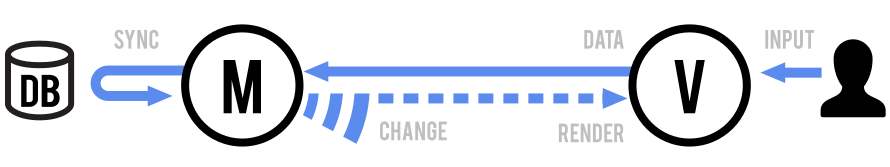
\includegraphics[scale=0.4]{Immagini/intro-model-view.png}
		\caption{Esempio MVC di Backbone}
	\end{figure}


La cosa più importante che Backbone può aiutarti è mantenere la business logic separata dall'user interface. Quando i due sono legati, cambiare è difficile; Quando la logica non dipende dall'interfaccia utente, è più facile lavorare con l'interfaccia.
\\
Model:
\begin{itemize}
\item Orchestra i dati e la business logic;
\item Carica e salva dal server;
\item Emette gli eventi quando i dati cambiano.
\end{itemize}
View:
\begin{itemize}
\item Ascolta le modifiche e renderizza l'UI;
\item Gestisce l'input dell'utente e l'interattività;
\item Comunica l'input catturato al modello.
\end{itemize}

Un model gestisce la tabella interna degli attributi dei dati e innesca gli eventi "modifica" quando uno dei suoi dati viene modificato.\\
I model gestiscono i dati di sincronizzazione con un livello di persistenza - di solito API REST con un database di backup. Progettate i model come oggetti riutilizzabili atomici che contengono tutte le funzioni utili per manipolare il loro particolare bit di dati. I model dovrebbero essere in grado di essere passati in tutta l'app e utilizzare quel bit di dati ovunque è necessario.\\

Una View è un pezzo atomico dell'interfaccia utente. Spesso renderizza i dati da un model specifico o da un numero di model, ma le View possono anche essere pezzi senza dati di UI che si trovano da soli. I model dovrebbero essere generalmente ignari delle View. Invece, le View ascoltano gli eventi "modifica" del model e reagiscono o si ri-renderizzano in modo appropriato.


\end{document}